\documentclass{beamer}
\usepackage[russian]{babel}
\usetheme{metropolis}

\usepackage{amsthm}
\setbeamertemplate{theorems}[numbered]

\setbeamercolor{block title}{use=structure,fg=white,bg=gray!75!black}
\setbeamercolor{block body}{use=structure,fg=black,bg=gray!20!white}

\usepackage[T2A]{fontenc}
\usepackage[utf8]{inputenc}

\usepackage{hyphenat}
\usepackage{amsmath}
\usepackage{graphicx}

\AtBeginEnvironment{proof}{\renewcommand{\qedsymbol}{}}{}{}

\title{
Микроэкономика-I
}
\author{
Павел Андреянов, PhD
}

\begin{document}

\maketitle

\section{Бюджетное ограничение}

\begin{frame}{План}

Первая половина лекции посвящена интерпретации Метода Множителей Лагранжа. Формулировки теорем знать не обязательно, но хотелось бы, чтобы вы примерно представляли, что происходит когда вы его применяете. 

Также будут введены термины спроса и косвенной полезности, и некоторые сопутствующие определения и свойства.

Вторая половина лекции посвящена отработке техник поиска спроса и косвенной полезности во всех классических примерах.

\end{frame}


\section{Бюджетное ограничение}

\begin{frame}{Бюджетное ограничение}

Наиболее часто в нашем курсе будет встречаться линейное бюджетное ограничение:
$$ B(x,y) = p x + q y - I \leqslant 0$$

где $p, q$ это цены товаров, а $I$ это бюджет. 

На прошлой лекции мы уже тренировались его рисовать, опираясь на точки $(I/p, 0)$ и $(0, I/q)$, соответствующие случаю, когда все расходы тратятся на один из двух товаров.

\end{frame}

\begin{frame}{Бюджетное ограничение}

\begin{figure}[hbt]
\centering
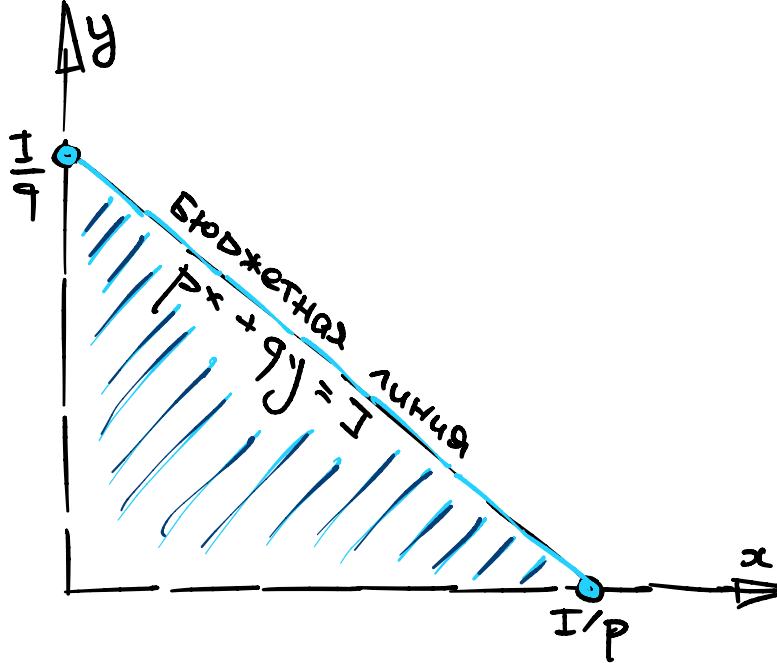
\includegraphics[width=.8 \textwidth]{budget_2d.png}
\end{figure}

\end{frame}

\section{Метод Лагранжа}

\begin{frame}{Метод Лагранжа}

Запишем нашу оптимизационную задачу в следующем виде:
$$ U(x, y) \to \max_{(x,y) \in \mathbb{R}^2_{+}} \quad s.t.\quad  B(x,y) \leqslant 0$$

Тогда Лагранжиан принимает вид:
$$ \mathcal{L}(x, y | \lambda) = U(x,y) - \lambda B(x,y)$$

Знак перед множителем Лагранжа важен в доказательствах, но на практике  не играет роли и можно ставить любой.

Традиция такова, что $\lambda I$ должен войти с плюсом.

\end{frame}

\begin{frame}{Метод Лагранжа}

Далее алгоритм предписывает найти безусловный экстремум Лагранжиана в пространстве $(x, y, \lambda)$, игнорируя ограничения.
$$ \mathcal{L}'_x = 0, \quad \mathcal{L}'_y = 0, \quad \mathcal{L}'_{\lambda} = 0.$$
Это система из трех уравнений с тремя неизвестными.

Таким образом, задача условной оптимизации сводится к безусловной. Однако, не совсем понятно, почему метод Лагранжа вообще работает и что он находит.

\end{frame}

\section{Выпуклая интерпретация ММЛ}

\begin{frame}{Выпуклая интерпретация ММЛ}

Если Лагранжиан (квази) вогнутый по товарам $x,y$ то можно применить, так называемый, \textbf{Сильный Принцип Лагранжа}:
$$ \min_{\lambda \geqslant 0} \max_{x(\lambda),y(\lambda) \geqslant 0} \mathcal{L}(x,y | \lambda) = \textcolor{red}{\max_{x,y \geqslant 0} \min_{\lambda(x,y) \geqslant 0} \mathcal{L}(x,y | \lambda)} $$ 

Справа стоит негладкая задача, эквивалентная условной оптимизации, поскольку $\lambda(x,y)$ выбирается так, чтобы наказать бесконечно отрицательной полезностью в случае выхода за ограничение.

\end{frame}

\begin{frame}{Выпуклая интерпретация ММЛ}

Если Лагранжиан (квази) вогнутый по товарам $x,y$ то можно применить, так называемый, \textbf{Сильный Принцип Лагранжа}:
$$ \textcolor{red}{\min_{\lambda \geqslant 0} \max_{x(\lambda),y(\lambda) \geqslant 0} \mathcal{L}(x,y | \lambda)} =  \max_{x,y \geqslant 0} \min_{\lambda(x,y) \geqslant 0} \mathcal{L}(x,y | \lambda) $$ 

Слева стоит гладкая задача, у которой есть один экстремум типа <<седло>>, а значит его можно найти обыкновенными условиями первого порядка:
$$ \nabla_{(x,y)} \mathcal{L} = 0, \quad \nabla_{\lambda} \mathcal{L} = 0.$$

В выпуклом случае, координаты решения двух задач, а также, значение целевой функции совпадают. Это называется \textbf{Теоремой о Минимаксе}, или \textbf{Сильной Дуальностью}.

\end{frame}

\section{Невыпуклая интерпретация ММЛ}

\begin{frame}{Невыпуклая интерпретация ММЛ}

В общем случае, технология поиска оптимума опирается на, так называемые, \textbf{условия Каруш-Кун-Такера}. Основная идея такова, что градиент целевой функции и градиент активного ограничения должны быть параллельны друг другу:
$$ \nabla_{(x,y)}U - \lambda \nabla_{(x,y)} B = 0$$

Это называется необходимыми условиями первого порядка. Удивительным образом, это совпадает с поиском седла Лагранжиана. Также, там есть условия невязки, о которых я упомяну чуть позже.

\end{frame}

\begin{frame}{Невыпуклая интерпретация ММЛ}

В общем случае, технология поиска оптимума опирается на, так называемые, \textbf{условия Каруш-Кун-Такера}. 

Основная идея такова, что градиент целевой функции и градиент активного ограничения должны быть параллельны друг другу:
$$ \nabla_{(x,y)}U - \lambda \nabla_{(x,y)} B = 0$$

Это называется необходимыми условиями первого порядка, или сокращенно \textbf{УПП} (в англ. \textbf{FOC}). Удивительным образом, это совпадает с поиском седла Лагранжиана.

\end{frame}

\begin{frame}{Невыпуклая интерпретация ММЛ}

Далее надо сделать еще один шаг и проверить достаточные условия второго порядка, или сокращенно \textbf{УВП} (в англ. \textbf{SOC}):
$$ \nabla^2_{(x,y)}U - \lambda \nabla^2_{(x,y)} B \leqslant 0$$

на касательном к ограничении пространстве. Еще более удивительным образом, это совпадает с проверкой (как бы локально) квази вогнутости Лагранжиана в точке.

\end{frame}


\section{Угловые решения}

\begin{frame}{Угловые решения}

На самом деле, поскольку мы оптимизируем в $\mathbb{R}^n_{+}$ в Лагранжиан стоило бы добавить еще дополнительные члены, по одному на каждый товар. 
$$ \mathcal{L}(x,y | \lambda, \ldots) = U(x,y) - \lambda B(x,y) - \ldots$$

Однако, в экономических приложениях, как правило, решение внутреннее. А когда оно не внутреннее, его очень легко отыскать по координатам бюджетного ограничения.

\end{frame}

\section{Значение Лагранжиана в оптимуме}

\begin{frame}{Значение Лагранжиана в оптимуме}

Вспомним условие невязки из курса мат. анализа:

$$ \lambda^{\ast} B(x^{\ast},y^{\ast}) = 0.$$

Оно означает, что одно из двух обязательно верно: либо множитель Лагранжа равен нулю, либо оптимум достигается на границе бюджетного ограничения.

Это значит, что в оптимуме, значение Лагранжиана совпадает со значением целевой функцией:
$$ \mathcal{L}(x^{\ast}, y^{\ast} | \lambda^{\ast}) = U(x^{\ast}, y^{\ast}) - \lambda B(x^{\ast}, y^{\ast})$$ 

Это нам пригодится, когда мы будем изучать ее.

\end{frame}

\section{Интерпретация $\lambda$}

\begin{frame}{Интерпретация $\lambda$}

У множителя $\lambda$ в Лагранжиане есть особая интерпретация, это теневая цена нарушения ограничения:
$$\mathcal{L} = U(x,y) - \lambda B(x,y), \quad B(x,y) \leqslant 0$$ 
Если вам очень хочется выйти за ограничение, Лагранж разрешает вам это сделать, то придется дать (кому-то абстрактно) взятку размера $\lambda$. Рынок подстроится таким образом, что вы не захотите эту взятку давать. 

\end{frame}

\section{Кривые спроса}

\begin{frame}{Кривые спроса}

Нас будут интересовать координаты оптимума $x^{\ast}(p,q,I)$, $y^{\ast}(p,q,I)$ в задаче максимизации полезности, при бюджетном ограничении, как функции (кривые) от цен $p,q$ и бюджета $I$. 

Они также называются \textbf{функциями (кривыми) спроса}.

\begin{definition}
Кривые вида \textbf{цена-потребление} $x^{\ast}(p,q, \ldots)$, $y^{\ast}(p,q, \ldots)$ обычно называются просто кривыми спроса. Кривые вида \textbf{доход-потребление} $x^{\ast}(I, \ldots)$, $y^{\ast}(I, \ldots)$ иногда называются кривыми Энгеля.
\end{definition}

\end{frame}

\section{Нормальные и инфериорные товары}

\begin{frame}{Нормальные товары}

Сфокусируемся на наклонах этих кривых по соответствующим параметрам. Первым мы изучим наклон кривой Энгеля, то есть, кривой доход-потребление.

\begin{definition}
\textbf{Нормальными товарами} называются товары, кривые спроса которых монотонно возрастают по доходу, то есть:
$$\frac{\partial x^{\ast}}{\partial I} \geqslant 0.$$
\end{definition}
Проверка нормальности при аккуратно выведенных кривых спроса - это механическое упражнение в дифференцировании.  

\end{frame}

\begin{frame}{Инфериорные товары}

Считается, что большая часть товаров - нормальны, однако есть исключения. Например, хлеб, рис, консервы и другие товары первой необходимости иногда интерпретируются как инфериорными по отношению к красному мясу, рыбе, овощам. 

\begin{definition}
Товар у которого нормальность нарушается хотя бы при каких то значениях параметров то есть, 
$$\frac{\partial x^{\ast}}{\partial I} < 0,$$ 
называется \textbf{инфериорным} (при этих значениях параметров). 
\end{definition}
\end{frame}

\begin{frame}{Инфериорные товары}

Инфериорность, от англ. \textit{inferior}, означает что ваш товар $x$ является худшим по отношению к какому то другому товару $y$. 

Когда бюджет растет, вы тратите большую часть дохода на $y$, и меньшую на $x$, да так что в абсолютном значении потребление $x$ уменьшается. 

\begin{lemma}
Все товары не могут быть одновременно инфериорными, хотя бы один точно нормальный.
\end{lemma}

Для того, чтобы сломать нормальность $x$, обязательно должен быть хотя бы один не инфериорный товар $y$, по отношению к которому $x$ будет инфериорным.

\end{frame}

\begin{frame}{Доказательство}

Если бюджетное ограничение таково, что оптимум находится внутри, то небольшое изменение параметра $I$ не повлияет на оптимум. Если бюджетное ограничение таково, что оптимум находится на бюджетной линии, то дифференциируя $B(x,y)= 0$ по $I$ мы получаем: 
$$ p \frac{\partial x^{\ast}}{\partial I}  + q \frac{\partial y^{\ast}}{\partial I}  = 1.$$ 

Поскольку цены неотрицательные, то инфериорность всех товаров означает, что слева стоит отрицательное число, а справа единица. Противоречие.

\end{frame}

\section{Субституты и комплементы}

\begin{frame}{Субституты}

Считается, что многие товары в той или иной степени замещаемы, некоторые больше некоторые меньше. Некоторые пары товаров особенно выделяются в этом плане, например: пепси и кола, лыжи и сноуборд... Если цена одного такого товара в паре сильно вырастет, то спрос на второй товар скорее всего вырастет. Такие товары называются субститутами.

\begin{definition}
\textbf{Субститутами} (substitutes) называются пары товаров, кривые спроса которых монотонно возрастают по ценам друг друга, то есть, $x$ субститут к $y$, если $\frac{\partial x^{\ast}}{\partial q} \geqslant 0,$ a $y$ субститут к $x$, если $\frac{\partial y^{\ast}}{\partial p} \geqslant 0.$
\end{definition}

\end{frame}

\begin{frame}{Заголовок в газетах}

\textit{Необычайная засуха в Калифорнии привела к дефициту воды и подорожанию свежих апельсинов и мандаринов на 18\%. Производители соков (не только апельсиновых, но также яблочных и других) из импортных концентратов собрались на экстренное собрание для обсуждения мер предотвращения дефицита.}

Почему они так сделали?

\end{frame}

\begin{frame}{Комплементы}

У некоторых пар товаров наблюдается прямо противоположное свойство, их обычно покупают вместе, например: кайак и весло, компьютер и монитор...  Если цена одного такого товара в паре сильно вырастет, то спрос на второй товар скорее всего упадет. Такие товары называются комплементами.

\begin{definition}
\textbf{Комплементами} (complements) называются пары товаров, кривые спроса которых монотонно убывают по ценам друг друга, то есть, $x$ комплемент к $y$, если $\frac{\partial x^{\ast}}{\partial q} < 0,$ a $y$ комплемент к $x$, если $\frac{\partial y^{\ast}}{\partial p} < 0.$
\end{definition}

\end{frame}

\begin{frame}{Заголовок в газетах}

\textit{Компания Самсунг отозвала крупную партию смартфонов, в связи с браком в производстве. Чтобы удержать долю на рынке, цены на основную линейку  смартфонов были уменьшены 25\%. Компания-производитель чехлов для смартфонов Самсунг неожиданно оказалась в списке единорогов.}

Что произошло?

\end{frame}

\begin{frame}{Мысли вслух}

К сожалению, субституты/комплементы не является симметричным свойством, то есть, $x$ может быть субститутом к $y$, но y при этом может оказаться комплементом к $x$, хоть и в очень редких случаях. 

Это сигнализирует нам о том, что определение выбрано не совсем удачно. Мы к этому вернемся в лекции 4.

Также, обратите внимание, что мы смотрели на наклоны кривых цена-потребление по не своим ценам: $x$ по $q$, $y$ по $p$. Наклон кривой спроса по собственной цене - это более сложный феномен, мы также к этому вернемся в лекции 4.

\end{frame}

\section{Косвенная полезность}

\begin{frame}{Косвенная полезность}

В каждой задаче оптимизации есть два объекта, идущие рука об руку: координаты оптимума и значение целевой функции (полезности). Мы довольно много внимания уделили координатам оптимума, то есть кривым спроса. 

А как насчет второго?

\begin{definition}
Назовем \textbf{косвенной полезностью} значение целевой функции в оптимуме, в задаче максимизации полезности:
$$ V(p,q,I) = U(x^{\ast}, y^{\ast}).$$
\end{definition}
Иногда я могу также использовать символ $U^{\ast}$.

\end{frame}

\begin{frame}{Косвенная полезность}

На самом деле, не столь важно какой буквой обозначается косвенная полезность: $U^{\ast}$ или $V$. Гораздо важнее набор аргументов: $p,q, I$, подсказывающий что координатам $x,y$ были присвоены какие то значения в процессе оптимизации.


Внимание! В отличие от координат оптимума, косвенная полезность, конечно же зависит от всех монотонных преобразований, которые вы наложили на свою полезность.

Если вы применили преобразование, например, $\log x$ чтобы быстрее решить задачу, и получили косвенную полезность, то вам придется ее откатить, то есть применить к ней обратное преобразование $e^x$, чтобы ответ был формально верным.

\end{frame}

\section{Непрерывность спроса}

\begin{frame}{Непрерывность спроса}

В большей часть примеров, которые мы будем рассматривать, спросы будут выражаться через элементарные функции, такие как $x^2, \log x, 1/x$... Все эти функции непрерывны. Совпадение?

Ответить на этот вопрос нам поможет \textbf{Теорема Максимума}: в \textbf{строго выпуклой} задаче оптимизации, решение, если оно существует, то единственно. Более того, если \textbf{задача непрерывна} по параметрам, то как координаты оптимума так и значение целевой функции непрерывны по параметрам.

Я буду иногда пользоваться следующими неформальными определениями: в строго выпуклой задаче, функция $U$ (квази) вогнутa, функция $B$ (квази) выпукла, причем одна из двух строго. В непрерывной задаче, обе функции $U$ и $B$ непрерывны.

\end{frame}

\section{Перерыв}



\end{document}